\documentclass[../../lectures.tex]{subfiles}

\begin{document}
\chapter{Виртуальная память}

\section{Прерывания и исключения}
\begin{itemize}
    \item Процессор с памятью не могут быть жить в вакууме (без ОС)
    \item Простыми словами: иногда процессор не знает что ему делать 
          в конкретной ситуации, так как не знает контекста исполнения, 
          тогда он просит помощи у внешней среды (чаще всего ОС)
    \item \emph{Interrupt Deriving Architecture} --- есть таблица, каждой ячейке 
          которой соотвествует какая-либо исключительная ситуация(например, 
          поделить на нуль) и функция ее разрешающая.
    \item \textbf{IDTR} --- регистр, в котором хранится адрес 
          \emph{Interrupt Descriptor Table} (глобальный)

          В некоторых архитектурах находится по фиксированному адресу 
          (например, x86 --- защищенный режим)

          Проще говоря \textbf{callbacks}

    \item Другой подход --- \emph{Polling} (есть управляющий код, 
          который периодически опрашивает устройство на предмет того,
          что нужно обработать; процессор выставляет флаг --- 
          "нуждаюсь в обработке"). 
          
          Пример --- сетевая карта

    \item У каждого подхода свои плюсы и минусы

    \item \textbf{CR2} --- контрольный регистр, считывается функцией \emph{do\_page\_fault} 
          (которая занимается обработкой \textbf{page fault})
\end{itemize}

\newpage
\section{Память}
\textbf{Проблемы памяти:}
\begin{enumerate}
    \item Памяти мало, она дорогая
    \item Памяти мало, программ много, как договориться?

          Закон Парето - 80\% обращений к 20\% памяти в среднем у пользовательской программы

          Может тогда выгружать неиспользуемую память на диск?

          Может еще переиспользовать память? (например, сегмент \textbf{text} у \textbf{chrome})
    \item Памяти мало, программ много, как защититься?

          Хочется чтобы каждый процесс был защищен от любого другого

          Неплохо было бы выложить в \emph{read-only} какую-то память 
          (сегмент \textbf{text} --- \emph{const}-переменные)

          \code{stackoverflow.cpp}{C++}

          Способ защиты --- память, которая может записываться не может выполняться

          Канарейка на стеке --- проверяем значение переменной 'канарейка', которую добавили после адреса возврата

          Хотим чтобы память ядра была недоступна пользователям
\end{enumerate}
\begin{center}\textbf{Как можно это все сделать?}\end{center}

\newpage
\section{Подходы к организации памяти}
\subsection{Досегментная организация}
Попробуем изменять адреса в программе перед запуском
\begin{itemize}
    \item Выделяем необходимое количество памяти
    \item Заменяем все адреса с учетом выделенной памяти
    \item \textbf{Relocations} --- механизм \todo{?}
    \item Проще говоря --- патчинг (но не всех страниц)
\end{itemize}
\textbf{Проблемы:}
\begin{itemize}
    \item А что, если нужно переместить программу в памяти?
    \item А что, если не найдем подходящего куска памяти?
    \item Нет защиты
\end{itemize}

\subsection{Сегментная организация}
Введем косвенность:
\begin{figure}[H]
\begin{minipage}[c]{0.5\linewidth}
\centering
\begin{itemize}
    \item Программы работают с виртуальными адресами
    \item Виртуальный адрес = смещение относительно сегмента
    \item Сегмент = база + размер
    \item Физический адрес = база сегмента + виртуальный адрес
    \item Перемещение памяти программы: изменение базы сегмента
    \item Переключение выполняемой программы: заменить поток выполнения + заменить сегмент
    \item Память per process
    \item \textbf{Relocations} все еще нужны
\end{itemize}
\end{minipage}
\hspace{0.5cm}
\begin{minipage}[c]{0.5\linewidth}
\centering
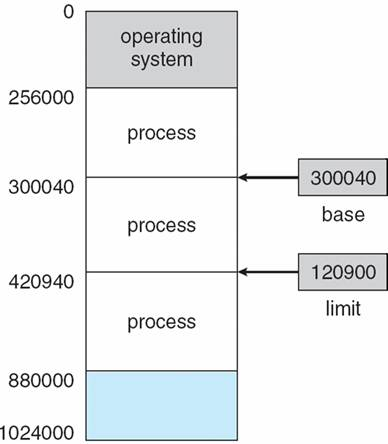
\includegraphics[width=\textwidth]{images/memory-segment.jpg}
\caption{Memory Segment}
\end{minipage}
\end{figure}

\begin{figure}[H]
\begin{minipage}[c]{0.6\linewidth}
\centering
\begin{itemize}
    \item Преобразование виртуального адреса в физический выполняет 
          \textbf{MMU} (Memory Managment Unit)
    \item \textbf{MMU} управляется из привилегированного режима
\end{itemize}
\end{minipage}
\hspace{0.5cm}
\begin{minipage}[c]{0.4\linewidth}
\centering
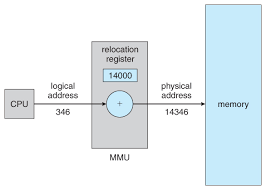
\includegraphics[width=\textwidth]{images/segment-translation.png}
\caption{Segment translation}
\end{minipage}
\end{figure}
\textbf{Плюсы:}
\begin{itemize}
    \item Быстро работает --- трансляция виртуального адреса в физический --- сложение, простое железо
          \centerimage{segmentation-hardware.jpg}{Segmentation Hardware}{0.4}
\end{itemize}
\textbf{Минусы:}
\begin{itemize}
    \item Сегмент имеет ограниченный размер - что если понадобилось больше памяти?
    \item Невозможность переиспользования памяти
    \item Несколько сегментов. x86 case study: \textbf{ds, ss, cs, general purpose}
          \begin{itemize}
              \item Добавляем права на сегменты
              \item Накладывает ограничения на модель работы
              \item Можно шарить память: сегменты кода или данных для чтения 
                    разных процессов одного исполняемого файла
                    имеют одинаковую базу и размер
              \item Усложнение логики \textbf{MMU}
          \end{itemize}
    \item Фрагментация: внешняя и внутренняя --- основная проблема
\end{itemize}

\subsection{Страничная организация}
\textbf{Как бороться с внешней фрагментацией?}
\begin{itemize}
    \item Нарежем все на кусочки --- страницы (в большинстве случаев ---  4KB)
    \item Размер страницы --- tradeoff внутренняя фрагментация и overhead
    \item Нужно уметь отображать виртуальный адрес страницы на физический --- \textbf{MMU}
    \item Ядро должно перехватывать ошибки обращений к страницам

          (Examples: write to read only, execute non executable)
    \item Ядро должно уметь изменять отображение виртуальных страниц в физические
\end{itemize}

\begin{figure}[H]
\begin{minipage}[c]{0.6\linewidth}
\centering
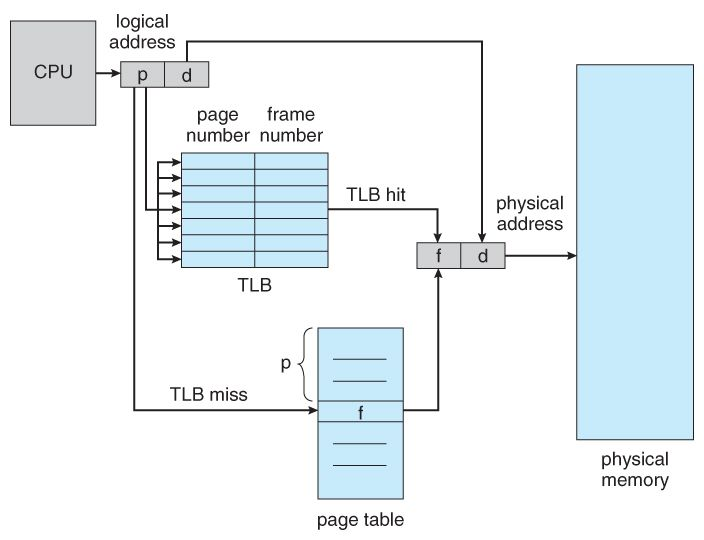
\includegraphics[width=\textwidth]{images/paging-hardware.jpg}
\caption{Paging hardware}
\end{minipage}
\hspace{0.5cm}
\begin{minipage}[c]{0.4\linewidth}
\centering
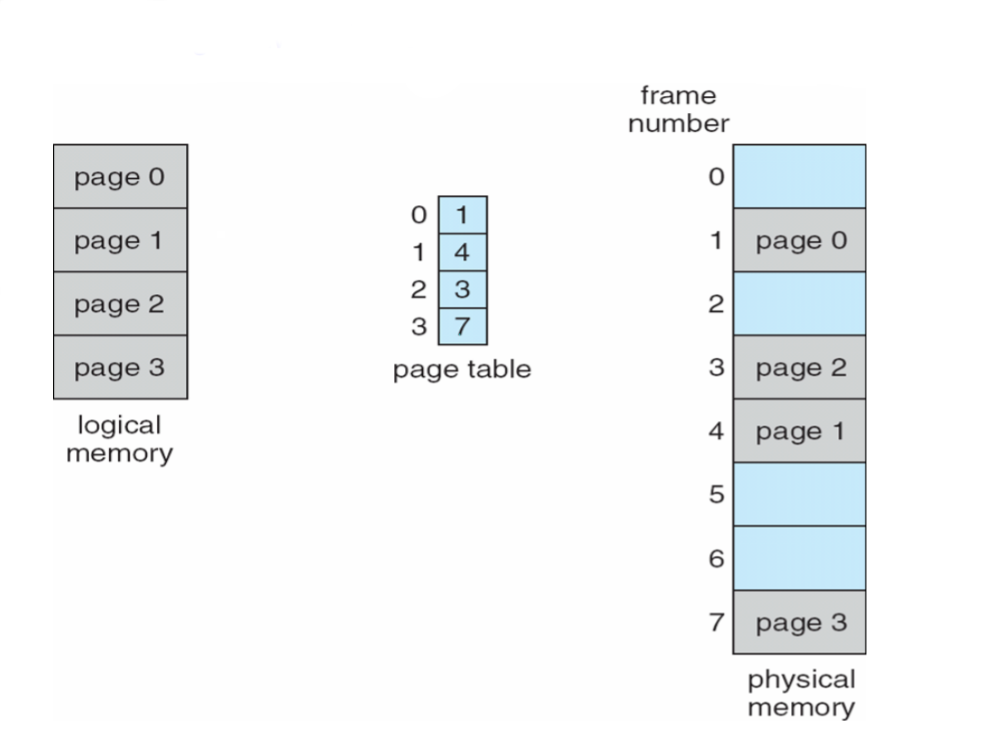
\includegraphics[width=\textwidth]{images/paging-addressing.png}
\caption{Paging addressing}
\end{minipage}
\end{figure}

\textbf{Тогда:}
\begin{itemize}
    \item Нет внешней фрагментации
    \item Внутренняя фрагментация --- half of page size
    \item Упрощается выделение памяти --- нужно найти не линейный кусок, а можно страницами
    \item Можно выгружать страницы памяти на диск
    \item Права можно задавать для каждой страницы отдельно
    \item Виртуальный адрес = номер страницы + смещение в странице
    \item Трансляция виртуального адреса --- трансляция адреса страницы + смещение в странице
    \item Процессу нужна таблица страниц
    \item У виртуального и физического адреса будут одинаковые --- \textbf{alignment}, \textbf{offset}
    \item Нам нужно хранить маппинг только для старших 20 бит.
\end{itemize}

\subsection{Страничная организация в x86}
\textbf{Чуть больше про реальность}
\begin{itemize}
    \item Таблица страниц - много места. Нужна иерархия.
    \item Размер иерархии - tradeoff между overhead на размер служебной информации и скоростью трансляции
    \item Иерархия:
          \begin{itemize}
              \item page directory = 1024 page directory entry (\textbf{PDE})
                    \begin{itemize}
                        \item \textbf{PDE} содержит адрес page table (\textbf{PT})
                    \end{itemize}
              \item \textbf{PT} --- 1024 page table entry (\textbf{PTE})
                    \begin{itemize}
                        \item \textbf{PTE} содержит физический адрес страницы
                        \item \textbf{PT} --- 4 MB of Virtual Memory
                    \end{itemize}
          \end{itemize}
    \item \textbf{CR3} --- контрольный регистр, хранящий физический адрес page directory
    \item В x86 одновременно есть и сегментация организация --- база в 0, размер на всю память
    \item x86-64 --- 4 уровня косвенности
    \item Время доступа --- дороже, в умных книжах пишут, что виртуальная память замедлила программы на 10---30\%
\end{itemize}

\begin{figure}[H]
\begin{minipage}[c]{0.5\linewidth}
\centering
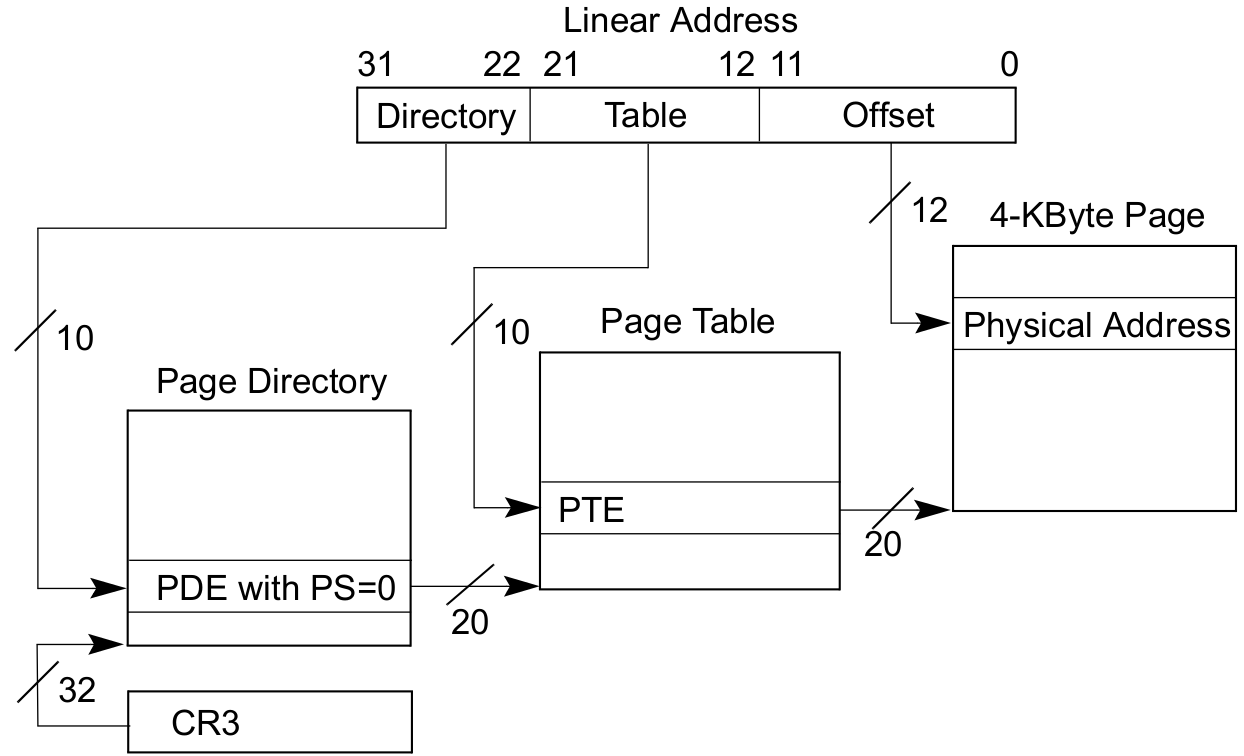
\includegraphics[width=\textwidth]{images/memory-x86-page-translation.png}
\caption{Page translation (x86)}
\end{minipage}
\hspace{0.5cm}
\begin{minipage}[c]{0.5\linewidth}
\centering
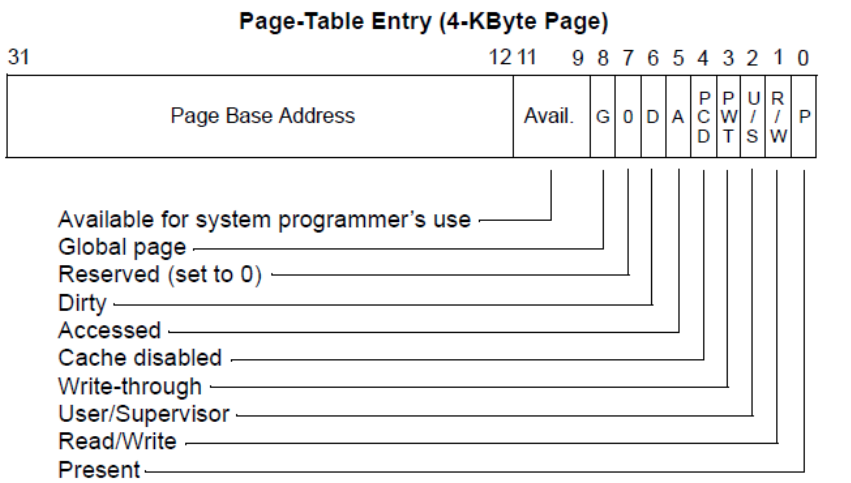
\includegraphics[width=\textwidth]{images/memory-pte.png}
\caption{Memory PTE}
\end{minipage}
\end{figure}

\section{MMU}
\begin{itemize}
    \item Трансляция выполняется аппаратно с помощью MMU
    \item Несколько обращений к памяти
    \item Проверка прав доступа
    \item Генерация прерываний при ошибках
    \item Медленно --- \textbf{TLB} (Translation Lookaside Buffer)
          \begin{itemize}
            \item Очень быстрый => очень дорогой => очень маленький
            \item Виртуальный адрес в физический
            \item Права доступа
            \item Инвалидация --- следит ядро
            \item \todo{paging-hardware?}
          \end{itemize}
\end{itemize}

\section{Переключение контекста}
\begin{itemize}
    \item Восстановить память процесса (регистр \textbf{CR3})
    \item Восстановить поток выполнения (значения регистров)
    \item Как защитить память ядра? --- привилегиями
\end{itemize}

\section{Page Fault}
\begin{itemize}
    \item Проверка \textbf{PD}, \textbf{PT}, \textbf{PTE}, прав доступа
    \item \textbf{MMU} генерирует прерывание --- адрес и тип доступа
    \item \textbf{ISR} в ядре
\end{itemize}
\todo{Картинка?}

\section{Page Reclaiming}
\begin{itemize}
    \item Идеальный --- нужно освободить ту страницу, которая дольше всего не потребуется
    \item Belady Anomaly
          \begin{itemize}
            \item \textbf{FIFO}
            \item Reference string: 1, 2, 3, 4, 1, 2, 5, 1, 2, 3, 4, 5
            \item 3 phys pages: 9 page faults
            \item 4 phys pages: 10 page faults
          \end{itemize}
    \item \textbf{LRU}
    \item Clock algorithm - aproximiate \textbf{LRU}
\end{itemize}
\todo{Картинка?}

\section{Примеры использования}
\subsection{Подкачка по требованию}
\begin{itemize}
    \item Пусть у нас есть фильм. Давайте читать этот файл используя
          окно считывания. Прикольно. Но можем замаппить файл в память 
          и читать его.
    \item Каждый раз когда читаем еще незагруженную страницу, \textbf{page fault},
          далее ядро подгружает страницу.
    \item Еще пример --- \shell{chrome \-\-help} (нам незачем инициализировать всю работу приложения)
    \item Ядро достаточно оптимально все это делает.
\end{itemize}
\subsection{Copy on write}
\code{copyonwrite.cpp}{C++}
Какое значение x будет в parent и в child?

Немного по-другому
\code{copyonwrite2.cpp}{C++}
\begin{itemize}
    \item Одинаковые адреса, значение разное (child --- 43, parent --- 42)
    \item При создании процесса --- ничего не делаем
    \item За всей этой истории стоит \textbf{MMU}
\end{itemize}

\subsection{Swap}
\begin{itemize}
    \item Скидывание на диск холодной data
    \item \textbf{MMU} ходит по кругу и проверяет использование страниц
\end{itemize}

\subsection{Другие}
\begin{itemize}
    \item Рост стека
    \item Разделяемый текст => Разделяемые библиотеки
    \item Разделяемая память
\end{itemize}

\section{Запрос памяти у ядра}
\subsection{Пример №1}
\code{mem1.c}{C}
\shell{cc mem1.c -o mem1}

\shell{strace -f ./mem1}
\code{mem1.trace}{C}

\begin{itemize}
    \item Нет никакого выделения памяти через \emph{malloc} (потому что это не системный вызов)
    \item \shell{man 2 brk, sbrk} --- явное увеличение/уменьшение кучи
    \item Для того же самого со стеком системных вызовов нет (только ассемблерные инструкции)
\end{itemize}

\subsection{Syscalls}
\begin{itemize}
    \item \emph{malloc/calloc/realloc} через прослойку выделяют себе блок памяти, режут его на куски и выдают клиенту-программисту
    \item \emph{free()} --- отдает блок памяти не ядру, а прослойке
    \item \emph{malloc()} --- неинициализированная память (сколько байт)
    \item \emph{calloc()} --- память инициализированная нулями (сколько объектов хотим)
    \item \emph{realloc()} --- все вместе (может еще перемещать память, 
          так как возвращается не всегда тот указатель, который передали)
    \item Операторы \textbf{new} и \textbf{delete} выражаются через функции C
\end{itemize}

\subsection{Helpers}
\begin{itemize}
    \item \textbf{Valgrind} --- выполняет инструкцию за инструкцией программы, которую ему передали 
          (строит внутри себя модель и отслеживает выделения памяти), долго работает 
          (значительно снижает производительность)
    \item \textbf{Sanitizer (ASAN)} --- инструментируют код, добавляют дополнительные проверки (тоже внутри себя строит модель)
    \item Программы с санитайзером работают не на порядок медленнее, а в 2-3 раза.
\end{itemize}

\subsection{Пример №2}
Когда мы делаем \emph{free()}, память может остаться в userspace.
\code{mem2.c}{C}
Что будет? --- \textbf{Undefined Behavior}

Но ведь ничего не напечаталось
\code{mem2.trace}{C}
На самом деле все напечаталось, просто мы этого не видим

\section{Mapping}

\subsection{Syscalls}
\emph{mmap(), munmap()}
\begin{itemize}
    \item Представьте, что у вас есть файл, и вы заранее не знаете к какой части файла будете обращаться.
    \item Замаппив этот файл в память своего процесса, нужно понимать, что ядро автомитечески не полностью подгружает его в память.
    \item Допустим, есть куча процессов, которые читают свой исполняемый файл\\
          Если бы мы делали это не через маппинг, то каждый раз надо было бы считывать что-то в локальные буфера
    \item С помощью маппинга можно избежать этой проблемы
\end{itemize}

\subsection{Пример №1}
\code{map1.c}{C}
\code{map1.trace}{C}
В выводе \emph{openat()}, так как мы делали не прямой системный вызов

\subsection{Пример №2}
Печать содержимого файла \textbf{/etc/passwd}
\code{map2.c}{C}
\code{map2.trace}{C}

\subsection{Additional}
\begin{itemize}
    \item \emph{pause()} --- системный вызов, останавливает программу, пока она не получит сигнал

    \item Ядро всегда зануляет память, которую отдает

    \item Как работают санитайзеры: выделяют справа и слева блоки памяти, 
          в которых устанавливают флаги и потом чекают на access к ним
\end{itemize}

\subsection{Пример №3}
\shell{man 2 mprotect}
\code{map3.c}{C}
\code{map3.trace}{C}

\shell{man 2 madvise}

\section{Аллокаторы памяти}
Зачем писать свой аллокатор памяти?

Случаи:
\begin{enumerate}
    \item Есть особенность данных, которую хотим использовать
    \item Когда нужно дебажить свой аллокатор
\end{enumerate}
\emph{Slab}-аллокаторы эксплуатируют то, что мы выделяем и освобождаем память одного и того же размера
\code{slab.c}{C}

\section{Безопасность}
\subsection{Meltdown}
\begin{itemize}
    \item Состоит из нескольких этапов
    \item Это атака позволяет читать непривилегированную для процесса память ядра
    \item Использует следующие особенности:
          \begin{itemize}
              \item Спекулятивное выполнение
              \item Утечка данных через сторонний канал
                  \begin{itemize}
                      \item Процессоры имеют кэши
                      \item Оценка времени доступа к массиву позволяет понять, находятся ли данные в кэше
                  \end{itemize}
          \end{itemize}
\end{itemize}

\subsection{ASLR}
Address space layout randomization
\code{aslr.c}{C}
Почему значения почти одинаковые при каждом запуске?

Они рандомизируются (еще один рубеж защиты)

\section{Литература}
\begin{itemize}
    \item Understanding the Linux Kernel by Daniel P. Bovet \& Marco Cesati

          (Достаточно хорошо описана архитектура)
    \item Intel 64 and IA-32 Architectures Software Developer's Manual Volume 3

          (Руководство от Intel)
    \item x86 Instruction Set Architecture by Tom Shanley

          (Выжимка руководства от Intel)
    \item What every programmer should know about memory by Ulrich Drepper

          (Очень полезно)
    \item Безопасное программирование на C и C++. Роберт С. Сиакорд

          (Про уязвимости)
\end{itemize}

\section{Домашнее задание №3}
Кусочек \textbf{JIT} компилятора

\textbf{Цель} --- получить знакомство с системными вызывами, используемыми для получения/освобождения
памяти от ядра. Получить представление о том, как может работать \textbf{JIT} компилятор.

\textbf{Программа должна}
\begin{itemize}
    \item Выделить память с помощью \emph{mmap(2)}.
    \item Записать в выделенную память машинный код, соответсвующий какой-либо функции.
    \item Изменить права на выделенную память - чтение и исполнение (\emph{mprotect(2)}).
    \item Вызвать функцию по указателю на выделенную память.
    \item Освободить выделенную память.
\end{itemize}

\textbf{Что может помочь?}
\begin{itemize}
    \item \shell{man objdump}
    \item help disassemble в \textbf{gdb}
\end{itemize}

\textbf{Extra points}
\begin{itemize}
    \item Сильные духом призываются к возможности модификации кода выполняемой функции
          в runtime. 
    \item Например, вы можете получить аргументом вызова вашей программы
          какое-то число и пропатчить машинный код этим числом. Эта часть задания будет
          оцениваться в дополнительные баллы.
\end{itemize}

\end{document}
